\chapter{Exploit 2}
\label{chap:exploit2}

So with the first exploit no longer working, I was determined to find another way. I started to message around on the HTB forums, to see if someone had found the same way; and could tell me what I was doing wrong. I got a response outlining another way to get a reverse shell into the server, so I started to work on that.

\vspace{3mm}

The blogpost from the first exploit also mentioned another file-read exploit with the email templates. However, there is another issue with the newsletter templates. Apparently, they are also capable of executing \verb|.phtml| files.

The initial exploit to gain admin access was the same, as I already expected. However, he (ab)uses the image-upload functionality given when you create a category. The instructions I got were quite bare, so I had to do some figuring out on how to exactly exploit this.

\vspace{3mm}

I started with a lot of DuckDuckGo-ing, figuring out how to include a malicious PHP script into an image. I found that there are two main\footnote{More information and two other ways: \\\url{https://hackers2devnull.blogspot.com/2013/05/how-to-shell-server-via-image-upload.html}} ways:

\begin{itemize}
    \item Firstly, you can add a small PHP script to the EXIF data of the image, basically giving it a description with a PHP script. The issue with this method is that this doesn't give a full reverse shell.
    \item Secondly, you can rename the PHP script, and try to trick the website into thinking you uploaded an image; whilst in reality it's a script. This can give a proper full shell, since you can upload any PHP script this way.
\end{itemize}

\begin{wrapfigure}{r}{3.5cm}
	\centering
	\captionsetup{justification=centering, font=small}
	\noindent 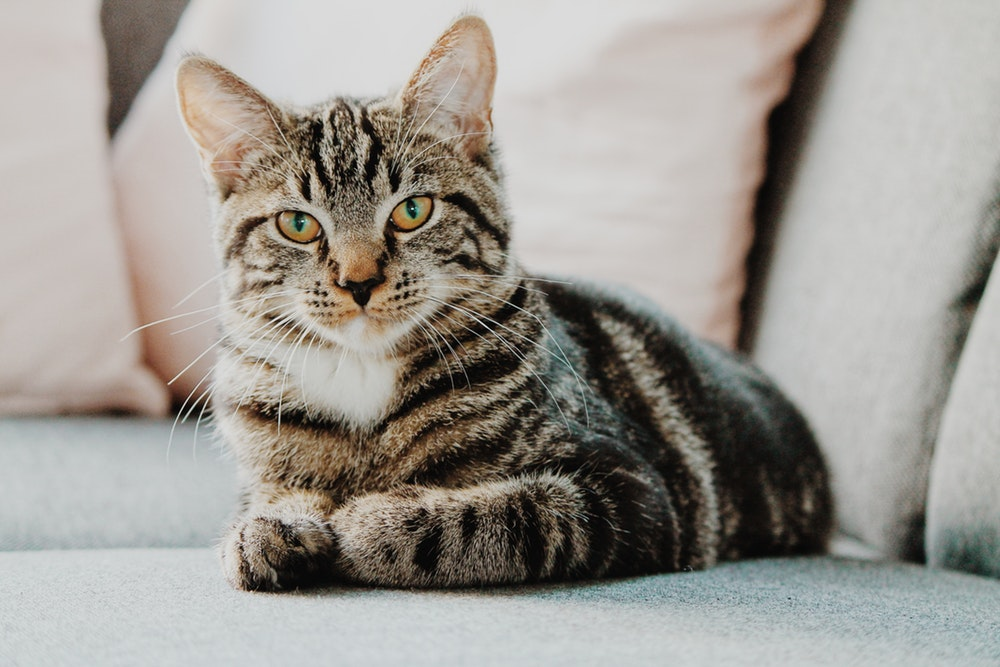
\includegraphics[width=\linewidth]{figures/cat.jpeg}
	\caption{\scriptsize{\emph{The cute cat picture I used for testing.}}}
	\label{fig:cat}
\end{wrapfigure}

So I decided to start with the second option, since it seemed like the easier one. I copied my reverse shell script a few times, using some of the suggestions from the blogpost found in the footnote. I uploaded them, but I wasn't sure if I'd get feedback from the site if it succeeded. Then I started to doubt whether the traversal from the second step would even work, so I used the cute cat picture seen in \cref{fig:cat} for a test.

Doing this, I found out that this trick indeed actually works. The raw image is displayed, indicating to me that this might be susceptible to executing code. After this I started to try more strange extensions, finding out that \verb|.php.jpg| worked. I knew this, because it showed up after I uploaded the file.

On to the second stage, the execution of the script. I got hinted towards another issue with the newsletter templates. Including the following code would allow me to traverse to the saved PHP script, and it should be executed via the 'Preview Template': 

\begin{Verbatim}[breaklines=true, breakanywhere=true]
    {{block type='core/template' template='../../../../../../media/catalog/category/reverse_shell.php.jpg}}
\end{Verbatim}

Another setting that needed to be changed was to allow symlinks. This setting can be found under \verb|System > Developer > Template Settings|. I suspect this allows the path traversing that is used in the path to the `image'.

The template could then be executed via the `Preview Template' option. This way, the server would show an iframe with the email content; including the `image'. The page would show an infinite loading screen, which is normal behavior for the reverse shell script.